\documentclass[a4paper, 12pt]{article}

% Русский язык
\usepackage[T2A]{fontenc}
\usepackage[utf8]{inputenc}
\usepackage[english,russian]{babel}

% Картинки
\usepackage{graphicx}
\graphicspath{{images/}}
\DeclareGraphicsExtensions{.pdf,.png,.jpg}
\usepackage{wrapfig}

% Математика
\usepackage{amsmath,amsfonts,amssymb,amsthm,mathtools} 

% Параметры страницы
\usepackage[left=2cm,right=2cm,top=2cm,bottom=3cm,bindingoffset=0cm]{geometry}

\usepackage{enumitem,xparse}
\usepackage{caption}
\usepackage{subcaption}
\usepackage{float}

\begin{document}

\newgeometry{left=2cm,right=2cm,top=2cm,bottom=1cm,bindingoffset=0cm}
\begin{titlepage}
    
    \begin{center}
        \vspace*{5cm}
        \Huge Московский Физико-Технический Институт
        \vspace*{2cm}\\
        \LARGE Отчет по эксперименту
        \\\vspace*{0.25cm}
        
        \noindent\rule{\textwidth}{1pt}
        \vspace*{-0.25cm}
        
        \huge \textbf{1.4.1-B\\ Изучение экспериментальных погрешностей на примере физического маятника}
        \noindent\rule{\textwidth}{1pt}


       \vfill
        \begin{flushright}
            \begin{minipage}{.4\textwidth}
            \Large Выполнил:\\ Студент 1 курса ФАКТ\\ Группа Б03-504 \\Подмосковнов Лев\\
            \end{minipage}
        \end{flushright}
        
        \vfill
        \normalsize Долгопрудный \\2025
        
    \end{center}
\end{titlepage}
\restoregeometry

\setcounter{page}{2}
\section*{Аннотация}
\noindent \textbf{Цель работы:} 1) на примере измерения периода свободных колебаний физического маятника познакомиться с систематическими и случайными погрешностями, прямыми и косвенными измерениями; 2) проверить справедливость формулы для периода колебаний физического маятника и определить значение ускорения свободного падения; 3) убедиться в справедливости теоремы Гюйгенса об обратимости точек опоры и центра качания маятника; 4) оценить погрешность прямых и косвенных измерений и конечного результата.

\noindent \textbf{В работе используются:} металлический стержень с опорной призмой; дополнительный груз; закреплённая на стене консоль; подставка с острой гранью для определения цента масс маятника; секундомер; счётчик колебаний (механический или электронный); линейки металлические различной длины; штангенциркуль; электронные весы; математический маятник (небольшой груз, подвешенный на нитях).

\section*{Теоритические сведения}

\[J=\frac{ml^2}{12}+ma^2\]

\[T=2\pi\sqrt{\frac{\frac{l^2}{12}+a^2}{ga}}\]

\[l_\text{пр}=a+\frac{l^2}{12a}\]

\[x_\text{ц}=\frac{m_0x_\text{ц0}+m_\text{г}y}{M}\]

\[T=2\pi\sqrt{\frac{J_0+m_\text{г}y^2}{gMx_\text{ц}}}\]

\section*{Оборудование и экспериментальные погрешности}

\noindent \textbf{Счётчик:} $\Delta_c=0,005c$

\noindent \textbf{Штангенциркуль:} $\Delta_{\text{шт}}=0,05\text{мм}$

\noindent \textbf{Весы:} $\Delta=0,005\text{г}$ 

\newpage

\section*{Результаты измерений и обработка данных}

\subsection*{Измерение длин и масс. Предварительный эксперимент}

\noindent \textbf{Максимальная систематическая погрешность:} $\varepsilon_{max}=0.1\%$

\noindent \textbf{Длина стержня:} $l=1000,0\text{мм}$

\noindent \textbf{Масса стержня:} $m=891,2\text{r}$

\noindent \textbf{Масса призмы:} $m_{\text{п}}=77,1\text{г}$

\noindent \textbf{Масса груза:} $m_{\text{п}}=314,0\text{г}$

\noindent \textbf{Положение острия призмы относительно центра масс стержня:} $a=243,0\text{мм}$

\noindent \textbf{Центр масс стержня с призмой:} $x_{\text{ц}}=482,0\text{мм}$

\begin{table}[!h]
\begin{center}
\begin{tabular}{|c|c|}
\hline
N опыта & t, c \\ \hline
1	& 30.78 \\ \hline
2	& 30.80 \\ \hline
3	& 30.74 \\ \hline
4	& 30.75 \\ \hline
5	& 30.74 \\ \hline
6	& 30.73 \\ \hline
7	& 30.78 \\ \hline
8	& 30.77 \\ \hline
9	& 30.77 \\ \hline
10	& 30.76 \\ \hline
\end{tabular}
\end{center}
\end{table}

\noindent \textbf{Период:} $T=1.568\text{с}$

\noindent \textbf{Период по формуле:} $T=1.567\text{c}$

\noindent \textbf{Ускорение свободного падения получилось:} $g=9.8\frac{\text{М}}{\text{С}^2}$

\begin{table}[!h]
\begin{center}
\begin{tabular}{|c|c|}
\hline
$\overline{t}$ & 30.76 c \\ \hline
$\sigma_{t}^{\text{случ}}$ & 0.02 c \\ \hline
$\sigma_{t}^{\text{сист}}$ & 0.01 c \\ \hline
$\sigma_{t}^{\text{полн}}$ & 0.02 c \\ \hline
\end{tabular}
\end{center}
\end{table}

\noindent \textbf{Число колебаний, по которому следует измерять период:} $n=16$

\newpage

\subsection*{Измерение периода колебаний при разных положениях груза}


\begin{table}[h]
\begin{center}
\begin{tabular}{|c|c|c|c|c|c|c|}
\hline
N опыта & $y$, мм & $x_\text{ц}$, мм & $n$ & $t_n$, с & $T$, c & $g$, м/c^2 \\ \hline
1 & 56  & 15 & 16 & 23.7  & 1.48 & 9.86\\ \hline
2 & 96  & 25 & 16 & 23.37 & 1.46 & 9.84\\ \hline
3 & 136 & 35 & 16 & 23.03 & 1.43 & 9.83\\ \hline
4 & 176 & 45 & 16 & 22.8  & 1.42 & 9.83\\ \hline
5 & 216 & 54 & 16 & 22.68 & 1.42 & 9.82\\ \hline
6 & 256 & 64 & 16 & 22.63 & 1.41 & 9.87\\ \hline
7 & 296 & 74 & 16 & 22.69 & 1.42 & 9.92\\ \hline
8 & 336 & 84 & 16 & 22.79 & 1.42 & 9.90\\ \hline
9 & 376 & 94 & 16 & 22.99 & 1.44 & 9.92\\ \hline
\end{tabular}
\end{center}
\end{table}

\begin{figure}[h]
    \centering
    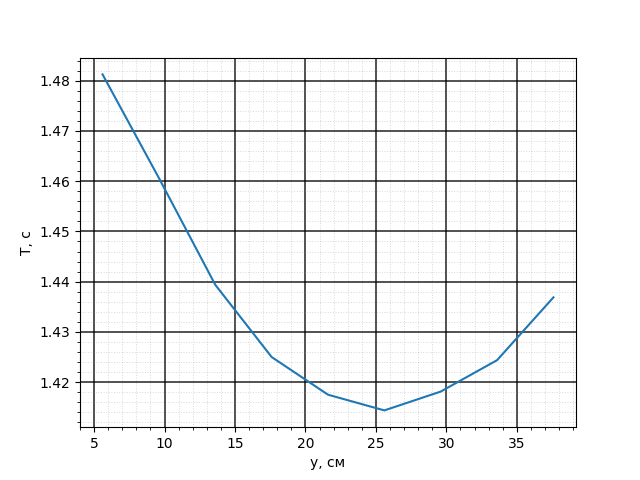
\includegraphics[width=0.8\textwidth]{1.png}
    \caption*{Зависимость периода от положения груза}
\end{figure}

\clearpage

\begin{figure}[h]
    \centering
    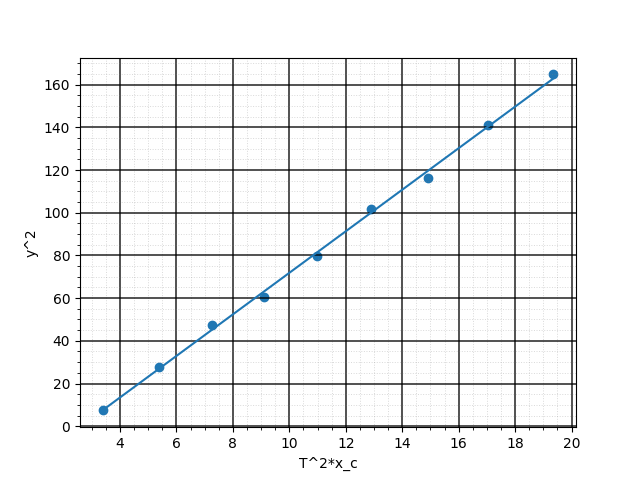
\includegraphics[width=0.8\textwidth]{2.png}
    \caption*{Зависимость $y^2$ от $T^2*x_\text{ц}$}
\end{figure}

Судя по графику $g$ = 9.73 м/с^2

$\sigma_k=0.14$

$\sigma_b = 0.02$

В итоге имеем следующие результаты для двух методов вычисления ускорения свободного
падения:

Непосредственное усреднение: $g=9.87\pm0.02$ м/с^2

Построение аппроксимирующей прямой: $g=9.73\pm0.14$ м/с^2

\subsection*{Провекра теоремы Гюйгенса}

$l_\text{пр}=57.8$мм

Для маятника без груза измерен период колебаний при подвесе его на расстоянии $l_\text{пр}$. Получено значение

$T_\text{пр}=(1,5245 \pm 0,005)$с

$T_0= (1,5245 \pm 0,005)$с

$T_\text{пр}=T_0$ в пределах погрешностей опыта. Следовательно, точка подвеса и центр качания физического маятника обратимы - теорема Гюйгенса подтвердилась.

\newpage

\section*{Вывод}

Данные значения лежат в пределах ≈ 1\% от табличных, что говорит о справедливости проверенных в работе закономерностей и формул. Однако разница значений и их погрешности не позволяют определить, в какой широте проводился опыт. Погрешность значения $g$ при прямом усреднении оказалась меньше, однако найденное таким методом значение больше отличается от табличного значения ускорения свободного падения в Московской области. Метод наименьших квадратов дал результат, более близкий к табличным значениям, однако отклонение всё равно заметное. Наиболее вероятным источником таким отклонений являются неучтённые систематические погрешности при определении центров масс стержня путём сбалансирования его на вспомогательной подставке. Для получения более точных данных следует, прежде всего, использовать более точные методы определения центра масс стержня.


\end{document}